% Please add the following required packages to your document preamble:
% \usepackage[normalem]{ulem}
% \useunder{\uline}{\ul}{}

\begin{table*}[]
    \begin{tabular}{|c|c|c|c|c|c|c|c|c|c|c|}
    \hline
    \textbf{\#}           & \textit{\textbf{1}}                                        & \textit{\textbf{2}}                                         & \textit{\textbf{3}}                                           & \textit{\textbf{4}}                                         & \textit{\textbf{5}}                                    & \textit{\textbf{6}}                                             & \textit{\textbf{7}}                                      & \textit{\textbf{8}}                                     & \textit{\textbf{9}}                                    & \textit{\textbf{10}}                                      \\ \hline
    \textit{Degree}       & Johann Sebastian Bach                                      & Traditional                                                 & Mc Gw                                                         & MC MN                                                       & Jean Sibelius                                          & Armin van Buuren                                                & Gucci Mane                                               & Steve Aoki                                              & Snoop Dogg                                             & Diplo                                                     \\ \hline
    \textit{Closeness}    & R3HAB                                                      & Snoop Dogg                                                  & Diplo                                                         & David Guetta                                                & Tiësto                                                 & Steve Aoki                                                      & Major Lazer                                              & Pitbull                                                 & Sean Paul                                              & French Montana                                            \\ \hline
    \textit{Betweenness}  & Snoop Dogg                                                 & Traditional                                                 & R3HAB                                                         & Diplo                                                       & Johann Sebastian Bach                                  & Tiësto                                                          & Major Lazer                                              & Steve Aoki                                              & Pitbull                                                & David Guetta                                              \\ \hline
    \textit{PageRank}     & Johann Sebastian Bach                                      & Traditional                                                 & Jean Sibelius                                                 & Mc Gw                                                       & MC MN                                                  & HaKokhav HaBa                                                       & John Williams                                            & A.R. Rahman                                             & Armin van Buuren                                       & Snoop Dogg                                                \\ \hline
    \textit{Eigenvector}  & Farruko                                                    & French Montana                                              & Gucci Mane                                                    & Ty Dolla \$ign                                              & Lil Wayne                                              & Chris Brown                                                     & Snoop Dogg                                               & De La Ghetto                                            & J Balvin                                               & Future                                                    \\ \hline
    \textit{Average rank} & \begin{tabular}[c]{@{}c@{}}Snoop Dogg\\ (5.8)\end{tabular} & \begin{tabular}[c]{@{}c@{}}Gucci Mane\\ (11.6)\end{tabular} & \begin{tabular}[c]{@{}c@{}}David Guetta\\ (18.8)\end{tabular} & \begin{tabular}[c]{@{}c@{}}Steve Aoki\\ (19.0)\end{tabular} & \begin{tabular}[c]{@{}c@{}}Diplo\\ (20.8)\end{tabular} & \begin{tabular}[c]{@{}c@{}}French Montana\\ (21.0)\end{tabular} & \begin{tabular}[c]{@{}c@{}}Pitbull\\ (23.4)\end{tabular} & \begin{tabular}[c]{@{}c@{}}Tiesto\\ (23.6)\end{tabular} & \begin{tabular}[c]{@{}c@{}}R3HAB\\ (24.4)\end{tabular} & \begin{tabular}[c]{@{}c@{}}The Game\\ (27.0)\end{tabular} \\ \hline
    \end{tabular}
    \caption{Top 10 artists in the whole dataset, according to our centrality measures. The "average rank" row also reports the value for each artist.}
    \label{tab:ranking}
    \end{table*}

\begin{table*}[]
    \centering
    \begin{tabular}{|c|c|c|c|c|c|c|c|}
    \hline
    \textbf{Reference graph}                                                       & \textit{Average cc} & \textit{Global cc} & \textit{\begin{tabular}[c]{@{}c@{}}Approximate\\ global cc\end{tabular}} & \textit{\begin{tabular}[c]{@{}c@{}}Maximum\\ eigenvector\end{tabular}} & \textit{\begin{tabular}[c]{@{}c@{}}Average\\ eigenvector\end{tabular}} & \textit{\begin{tabular}[c]{@{}c@{}}Maximum\\ closeness\end{tabular}} & \textit{\begin{tabular}[c]{@{}c@{}}Average\\ closeness\end{tabular}} \\ \hline
    \textbf{House subgraph}                                                        & \xmark              & \cmark             & \cmark                                                                   & \cmark                                                                 & \cmark                                                                 & \cmark                                                               & \cmark                                                               \\ \hline
    \textbf{Pop subgraph}                                                          & \xmark              & \xmark             & \xmark                                                                   & \cmark                                                                 & \cmark                                                                 &                                                                      &                                                                      \\ \hline
    \textbf{Rap subgraph}                                                          & \xmark              & \xmark             & \xmark                                                                   & \cmark                                                                 & \cmark                                                                 & \cmark                                                               & \xmark                                                               \\ \hline
    \textbf{Whole dataset}                                                         & \xmark              & \xmark             & \xmark                                                                   & \cmark                                                                 & \cmark                                                                 &                                                                      &                                                                      \\ \hline
    \textbf{\begin{tabular}[c]{@{}c@{}}Top 10\%\\ popularity subgraph\end{tabular}} & \xmark              & \xmark             & \xmark                                                                   & \cmark                                                                 & \cmark                                                                 & \xmark                                                               & \xmark                                                               \\ \hline
    \textbf{Trap subgraph}                                                         & \xmark              & \xmark             & \xmark                                                                   & \cmark                                                                 & \cmark                                                                 & \cmark                                                               & \xmark                                                               \\ \hline
    \end{tabular}
    \caption{Results of the Shapiro-Wilk normality tests for all considered graphs. The "reference graph" is the graph to which the random graphs used in the analysis refer to. "cc" stands for "clustering coefficient".}
    \label{tab:normality}
\end{table*}

\begin{table*}[]
  \centering
  \begin{tabular}{|c|c|c|c|c|c|c|c|}
  \hline
  \textbf{Reference graph}                                                        & \textit{Average cc}     & \textit{Global cc}   & \textit{\begin{tabular}[c]{@{}c@{}}Approximate\\ global cc\end{tabular}} & \textit{\begin{tabular}[c]{@{}c@{}}Maximum\\ eigenvector\end{tabular}} & \textit{\begin{tabular}[c]{@{}c@{}}Average\\ eigenvector\end{tabular}} & \textit{\begin{tabular}[c]{@{}c@{}}Maximum\\ closeness\end{tabular}} & \textit{\begin{tabular}[c]{@{}c@{}}Average\\ closeness\end{tabular}} \\ \hline
  \textbf{House subgraph}                                                         & \textbf{\textgreater{}} & \textbf{\textless{}} & \textbf{\textless{}}                                                     & \textbf{\textgreater{}}                                                & \textbf{\textgreater{}}                                                & \textbf{\textgreater{}}                                              & \textbf{\textgreater{}}                                              \\ \hline
  \textbf{Pop subgraph}                                                           & \textbf{\textgreater{}} & \textbf{\textless{}} & \textbf{\textless{}}                                                     & \textbf{\textgreater{}}                                                & \textbf{\textgreater{}}                                                & \textbf{}                                                            & \textbf{}                                                            \\ \hline
  \textbf{Rap subgraph}                                                           & \textbf{\textgreater{}} & \textbf{\textless{}} & \textbf{\textless{}}                                                     & \textbf{\textgreater{}}                                                & \textbf{\textgreater{}}                                                & \textbf{\textgreater{}}                                              & \textbf{\textgreater{}}                                              \\ \hline
  \textbf{Whole dataset}                                                          & \textbf{\textgreater{}} & \textbf{\textless{}} & \textbf{\textless{}}                                                     & \textbf{\textgreater{}}                                                & \textbf{\textless{}}                                                   & \textbf{}                                                            & \textbf{}                                                            \\ \hline
  \textbf{\begin{tabular}[c]{@{}c@{}}Top 10\%\\ popularity subgraph\end{tabular}} & \textbf{\textgreater{}} & \textbf{\textless{}} & \textbf{\textless{}}                                                     & \textbf{\textgreater{}}                                                & \textbf{\textgreater{}}                                                & \textbf{\textgreater{}}                                              & \textbf{\textgreater{}}                                              \\ \hline
  \textbf{Trap subgraph}                                                          & \textbf{\textgreater{}} & \textbf{\textless{}} & \textbf{\textless{}}                                                     & \textbf{\textgreater{}}                                                & \textbf{\textgreater{}}                                                & \textbf{\textgreater{}}                                              & \textbf{\textgreater{}}                                              \\ \hline
  \end{tabular}
  \caption{Results of the p-value computations: the contents of the cells represent how we should expect the metric values to be, compared to the values computed on the real (sub)graphs, if we were to accept our null hypothesis. "cc" stands for "clustering coefficient".}
  \label{tab:pvalue}
\end{table*}

\begin{figure*}
    \centering
    \begin{subfigure}{.33\textwidth}
      \centering
      \captionsetup{justification=centering}
      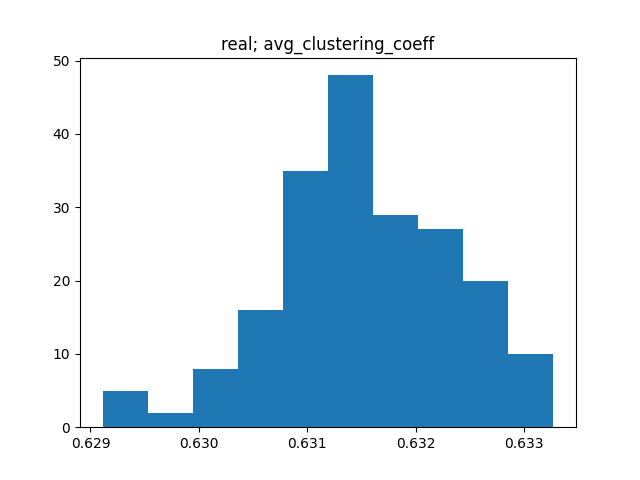
\includegraphics[width=\linewidth]{dist_plot_real_avg_clustering_coeff.png}
      \caption{Whole dataset, average \\ clustering coefficient}
      \label{fig:hist1}
    \end{subfigure}%
    \begin{subfigure}{.33\textwidth}
      \centering
      \captionsetup{justification=centering}
      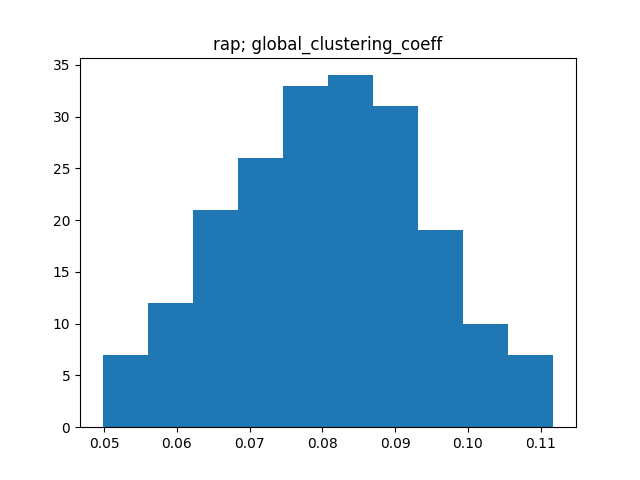
\includegraphics[width=\linewidth]{dist_plot_rap_global_clustering_coeff.png}
      \caption{Rap subgraph, global \\ clustering coefficient}
      \label{fig:hist2}
    \end{subfigure}
    \begin{subfigure}{.33\textwidth}
      \centering
      \captionsetup{justification=centering}
      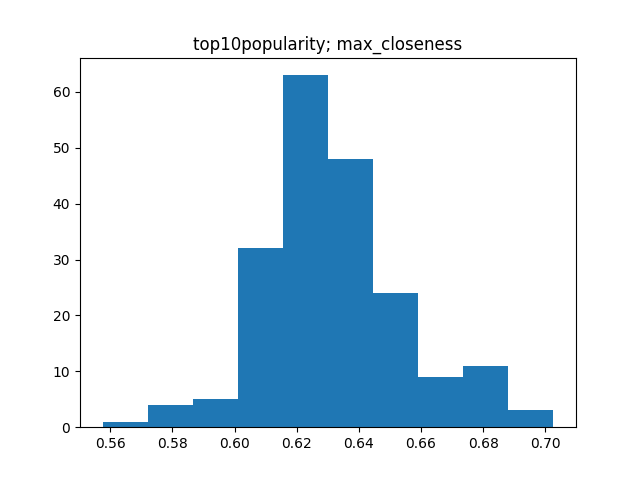
\includegraphics[width=\linewidth]{dist_plot_top10popularity_max_closeness.png}
      \caption{Top 10\% popularity subgraph, maximum closeness}
      \label{fig:hist3}
    \end{subfigure}
    \begin{subfigure}{.33\textwidth}
      \centering
      \captionsetup{justification=centering}
      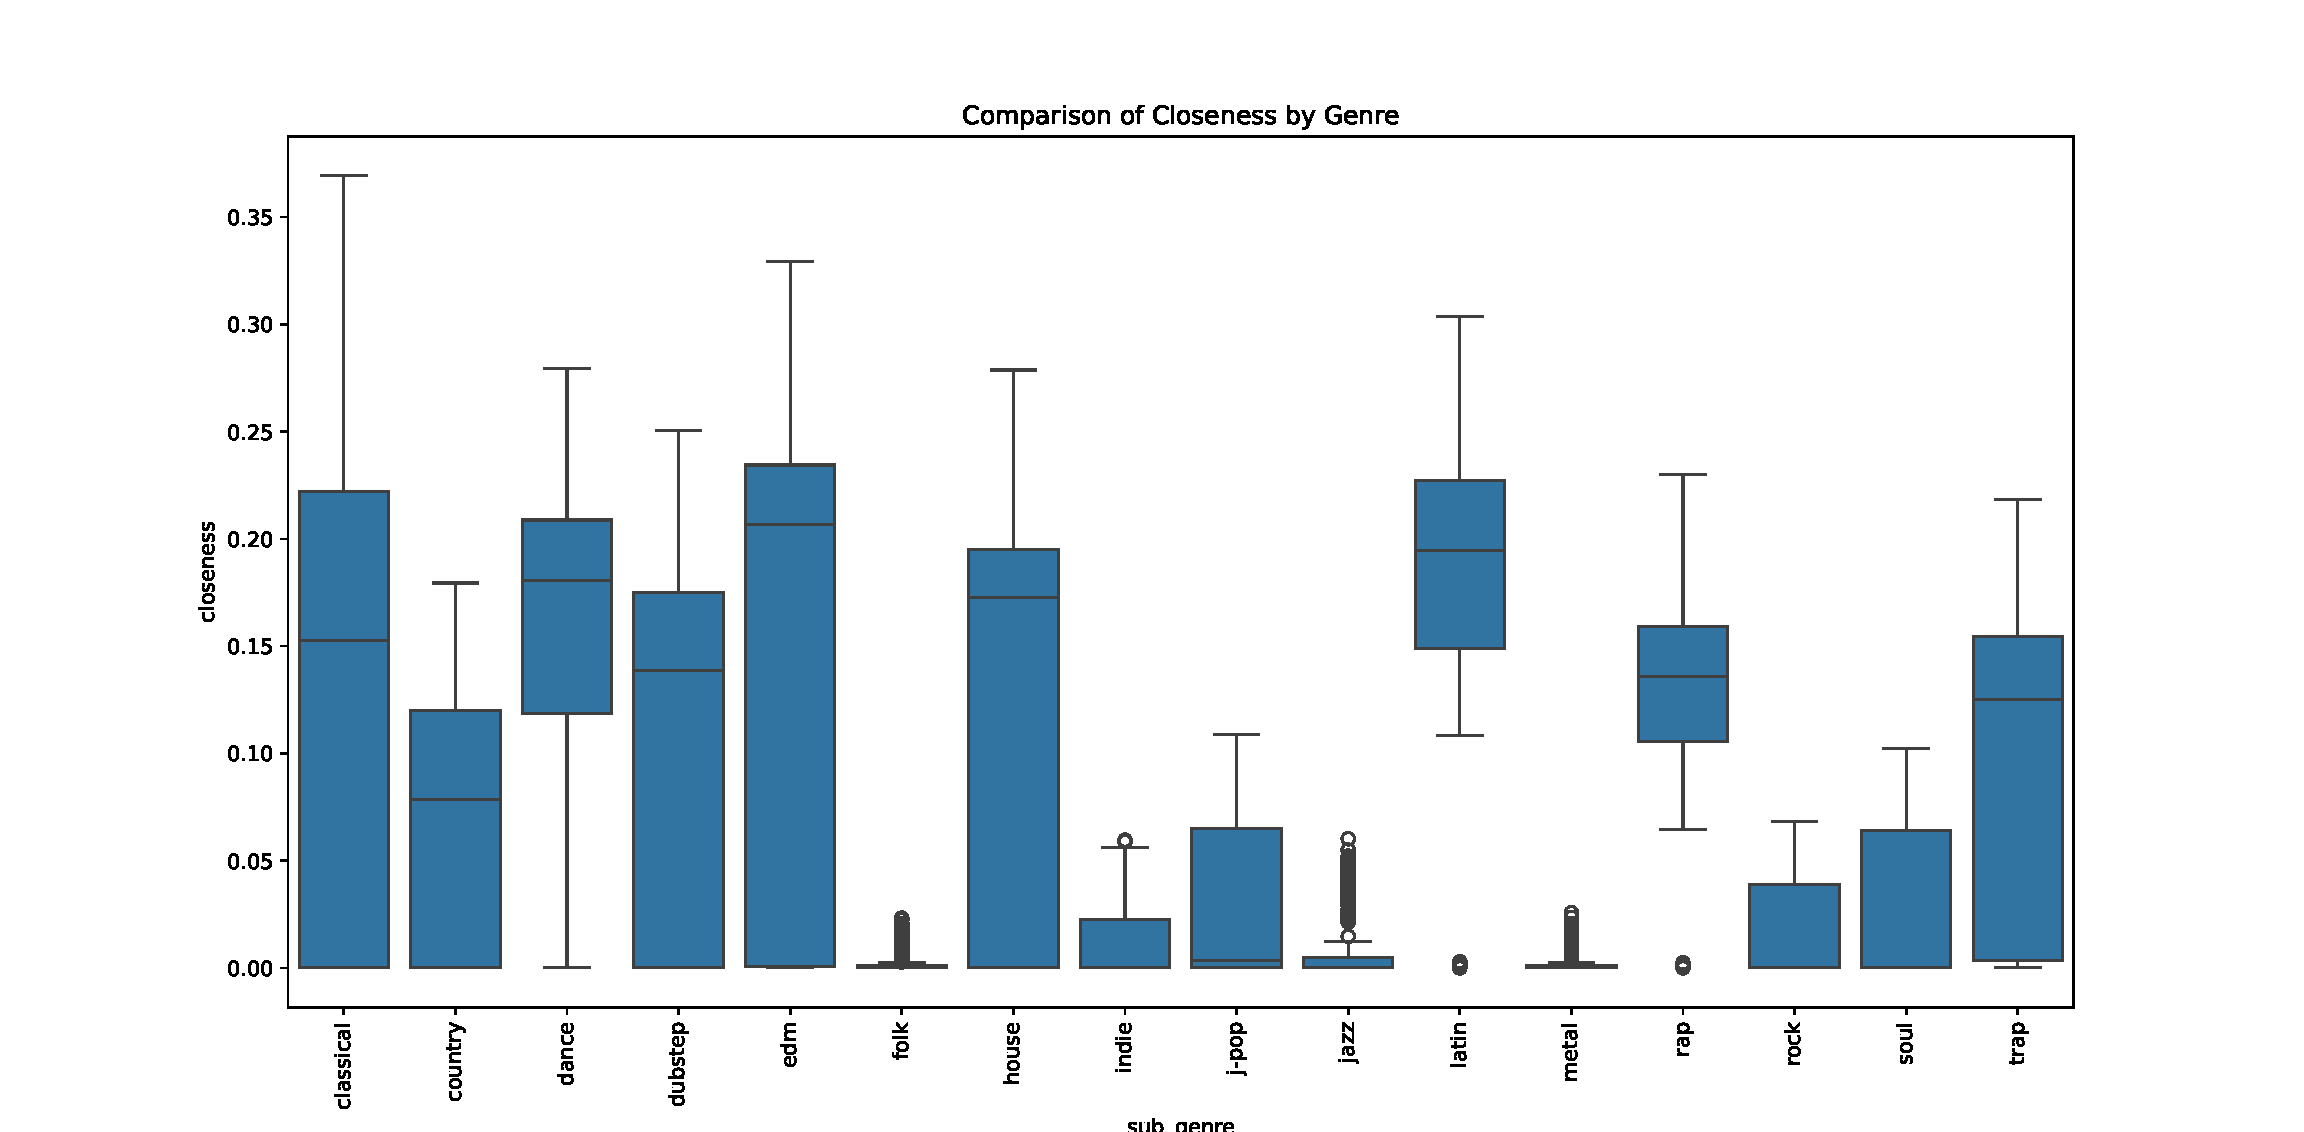
\includegraphics[width=\linewidth]{../../results/sub_genre/closeness.pdf}  % Usa \includegraphics per il PDF
      \caption{closeness plot}
      \label{fig:hist4}
    \end{subfigure}
    \begin{subfigure}{.33\textwidth}
      \centering
      \captionsetup{justification=centering}
      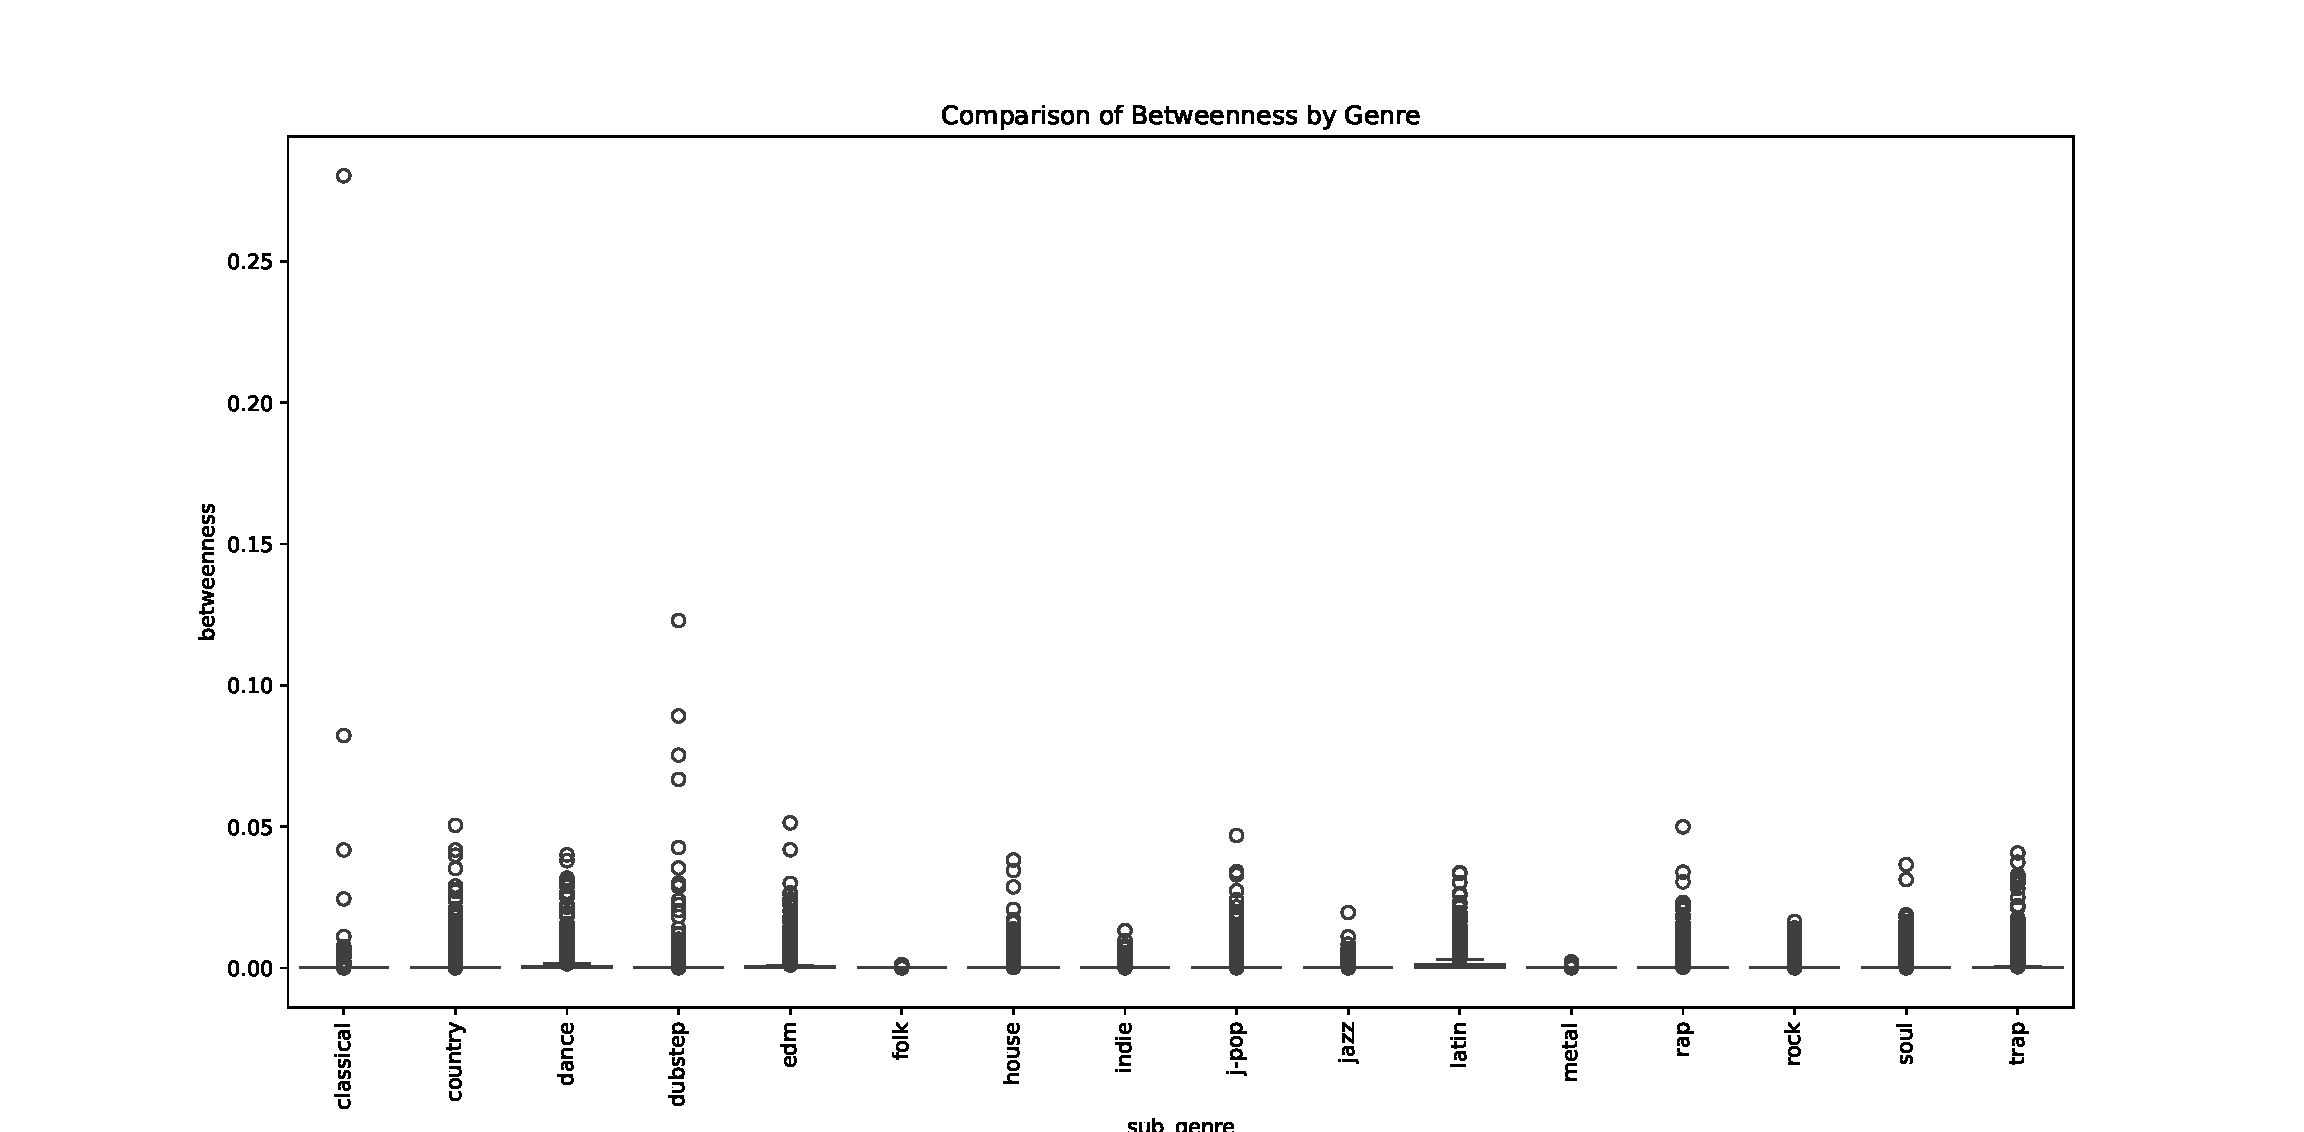
\includegraphics[width=\linewidth]{../../results/sub_genre/betweenness.pdf}  % Usa \includegraphics per il PDF
      \caption{betweenness plot}
      \label{fig:hist5}
    \end{subfigure}
    \begin{subfigure}{.33\textwidth}
      \centering
      \captionsetup{justification=centering}
      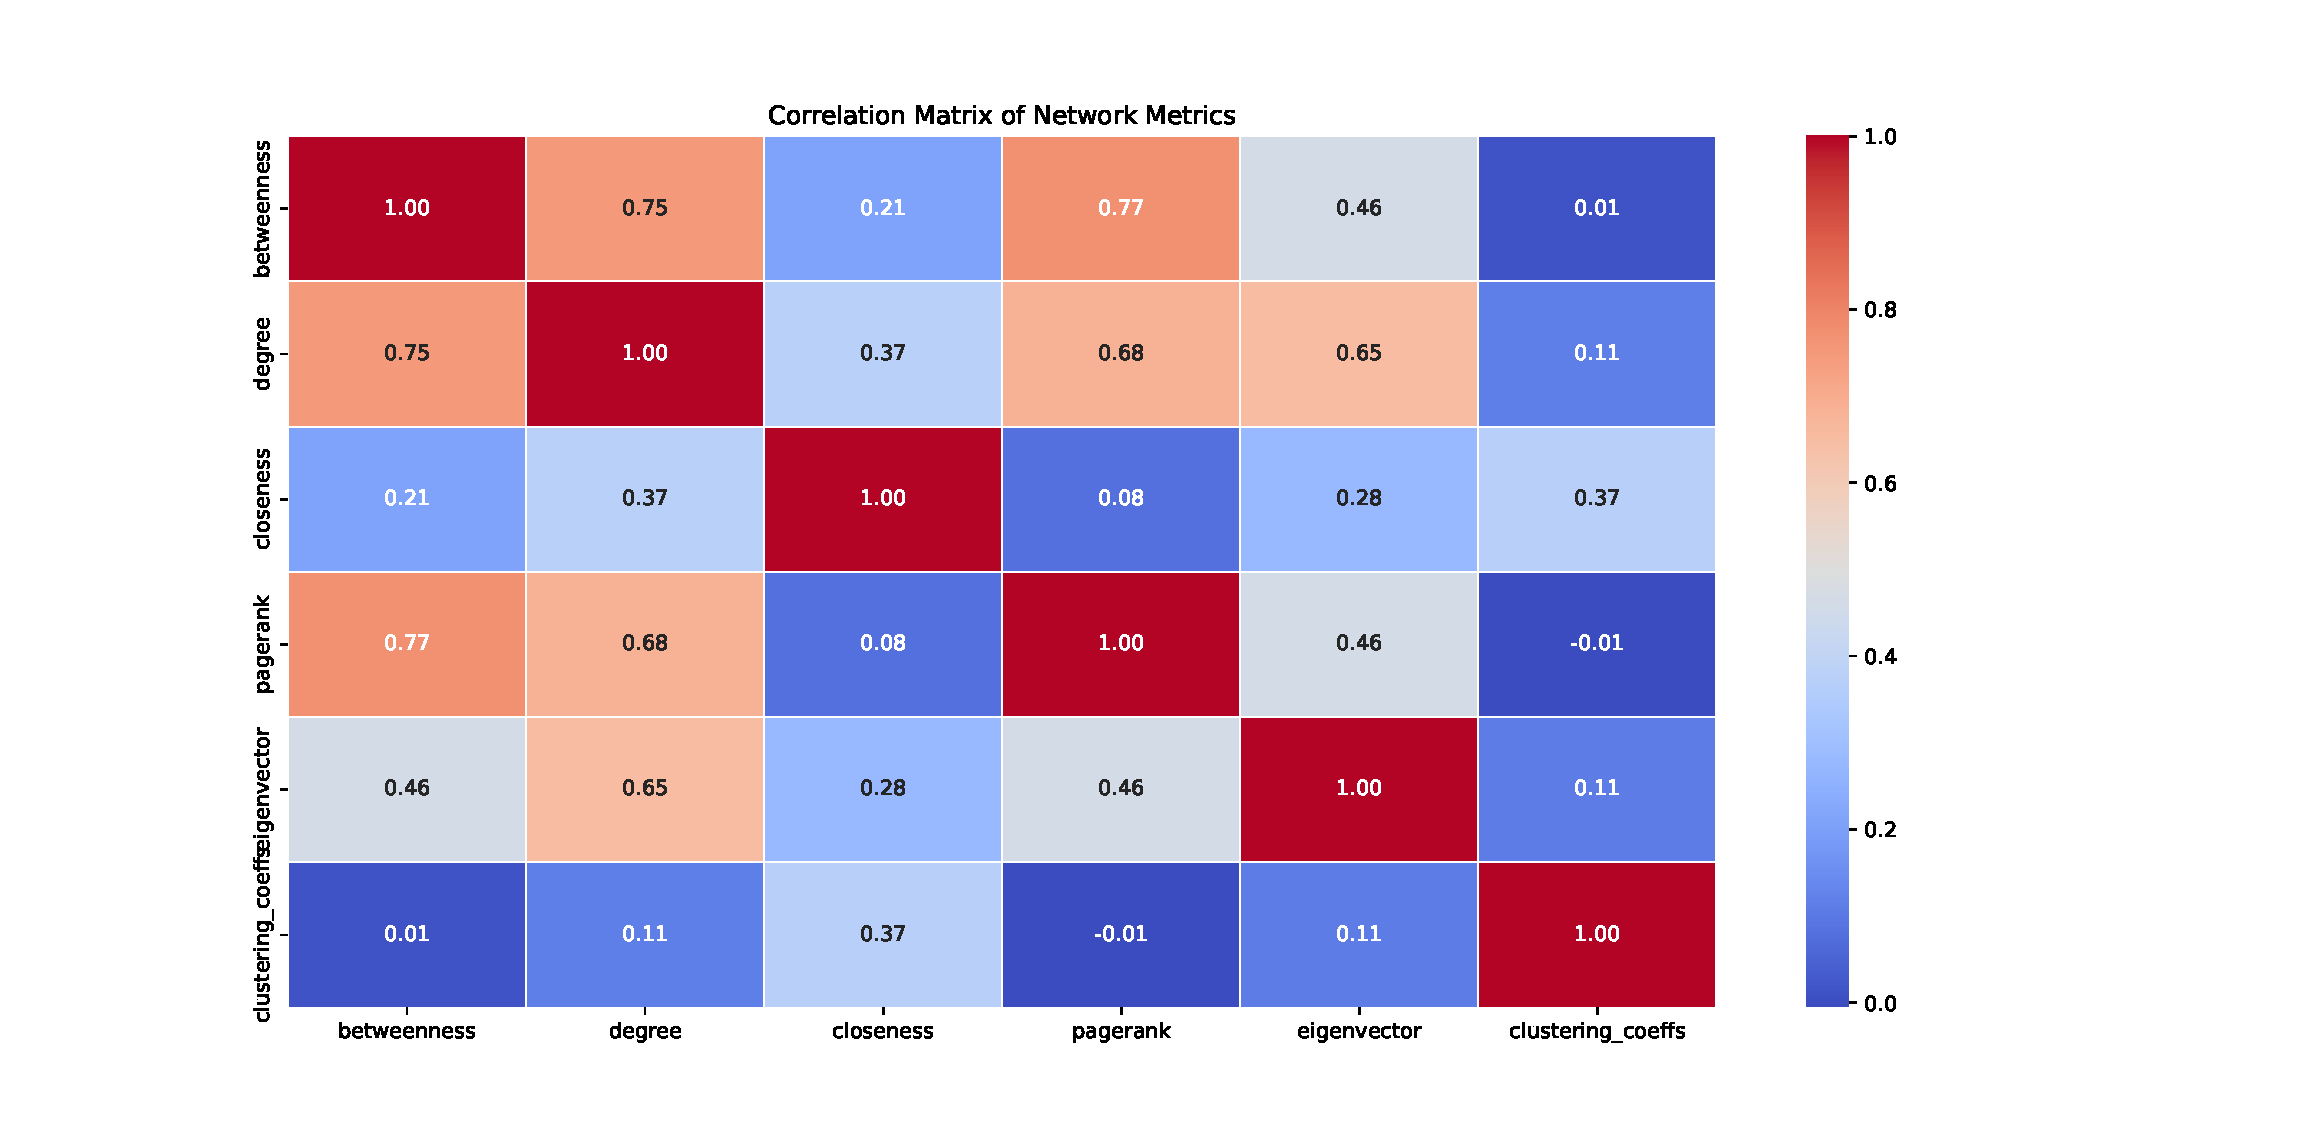
\includegraphics[width=1.25\linewidth, height=3cm]{../../results/sub_genre/correlation_matrix.pdf}  % Usa \includegraphics per il PDF
      \caption{Correlation Matrix}
      \label{fig:hist6}
    \end{subfigure}
    \caption{Example of histograms for the metrics computed on random graphs that do not have a Gaussian distribution according to the Shapiro-Wilk test.}
    \label{fig:hist}
\end{figure*}